\begin{Large}
	\vskip1cm
	\begin{figure}[h]
		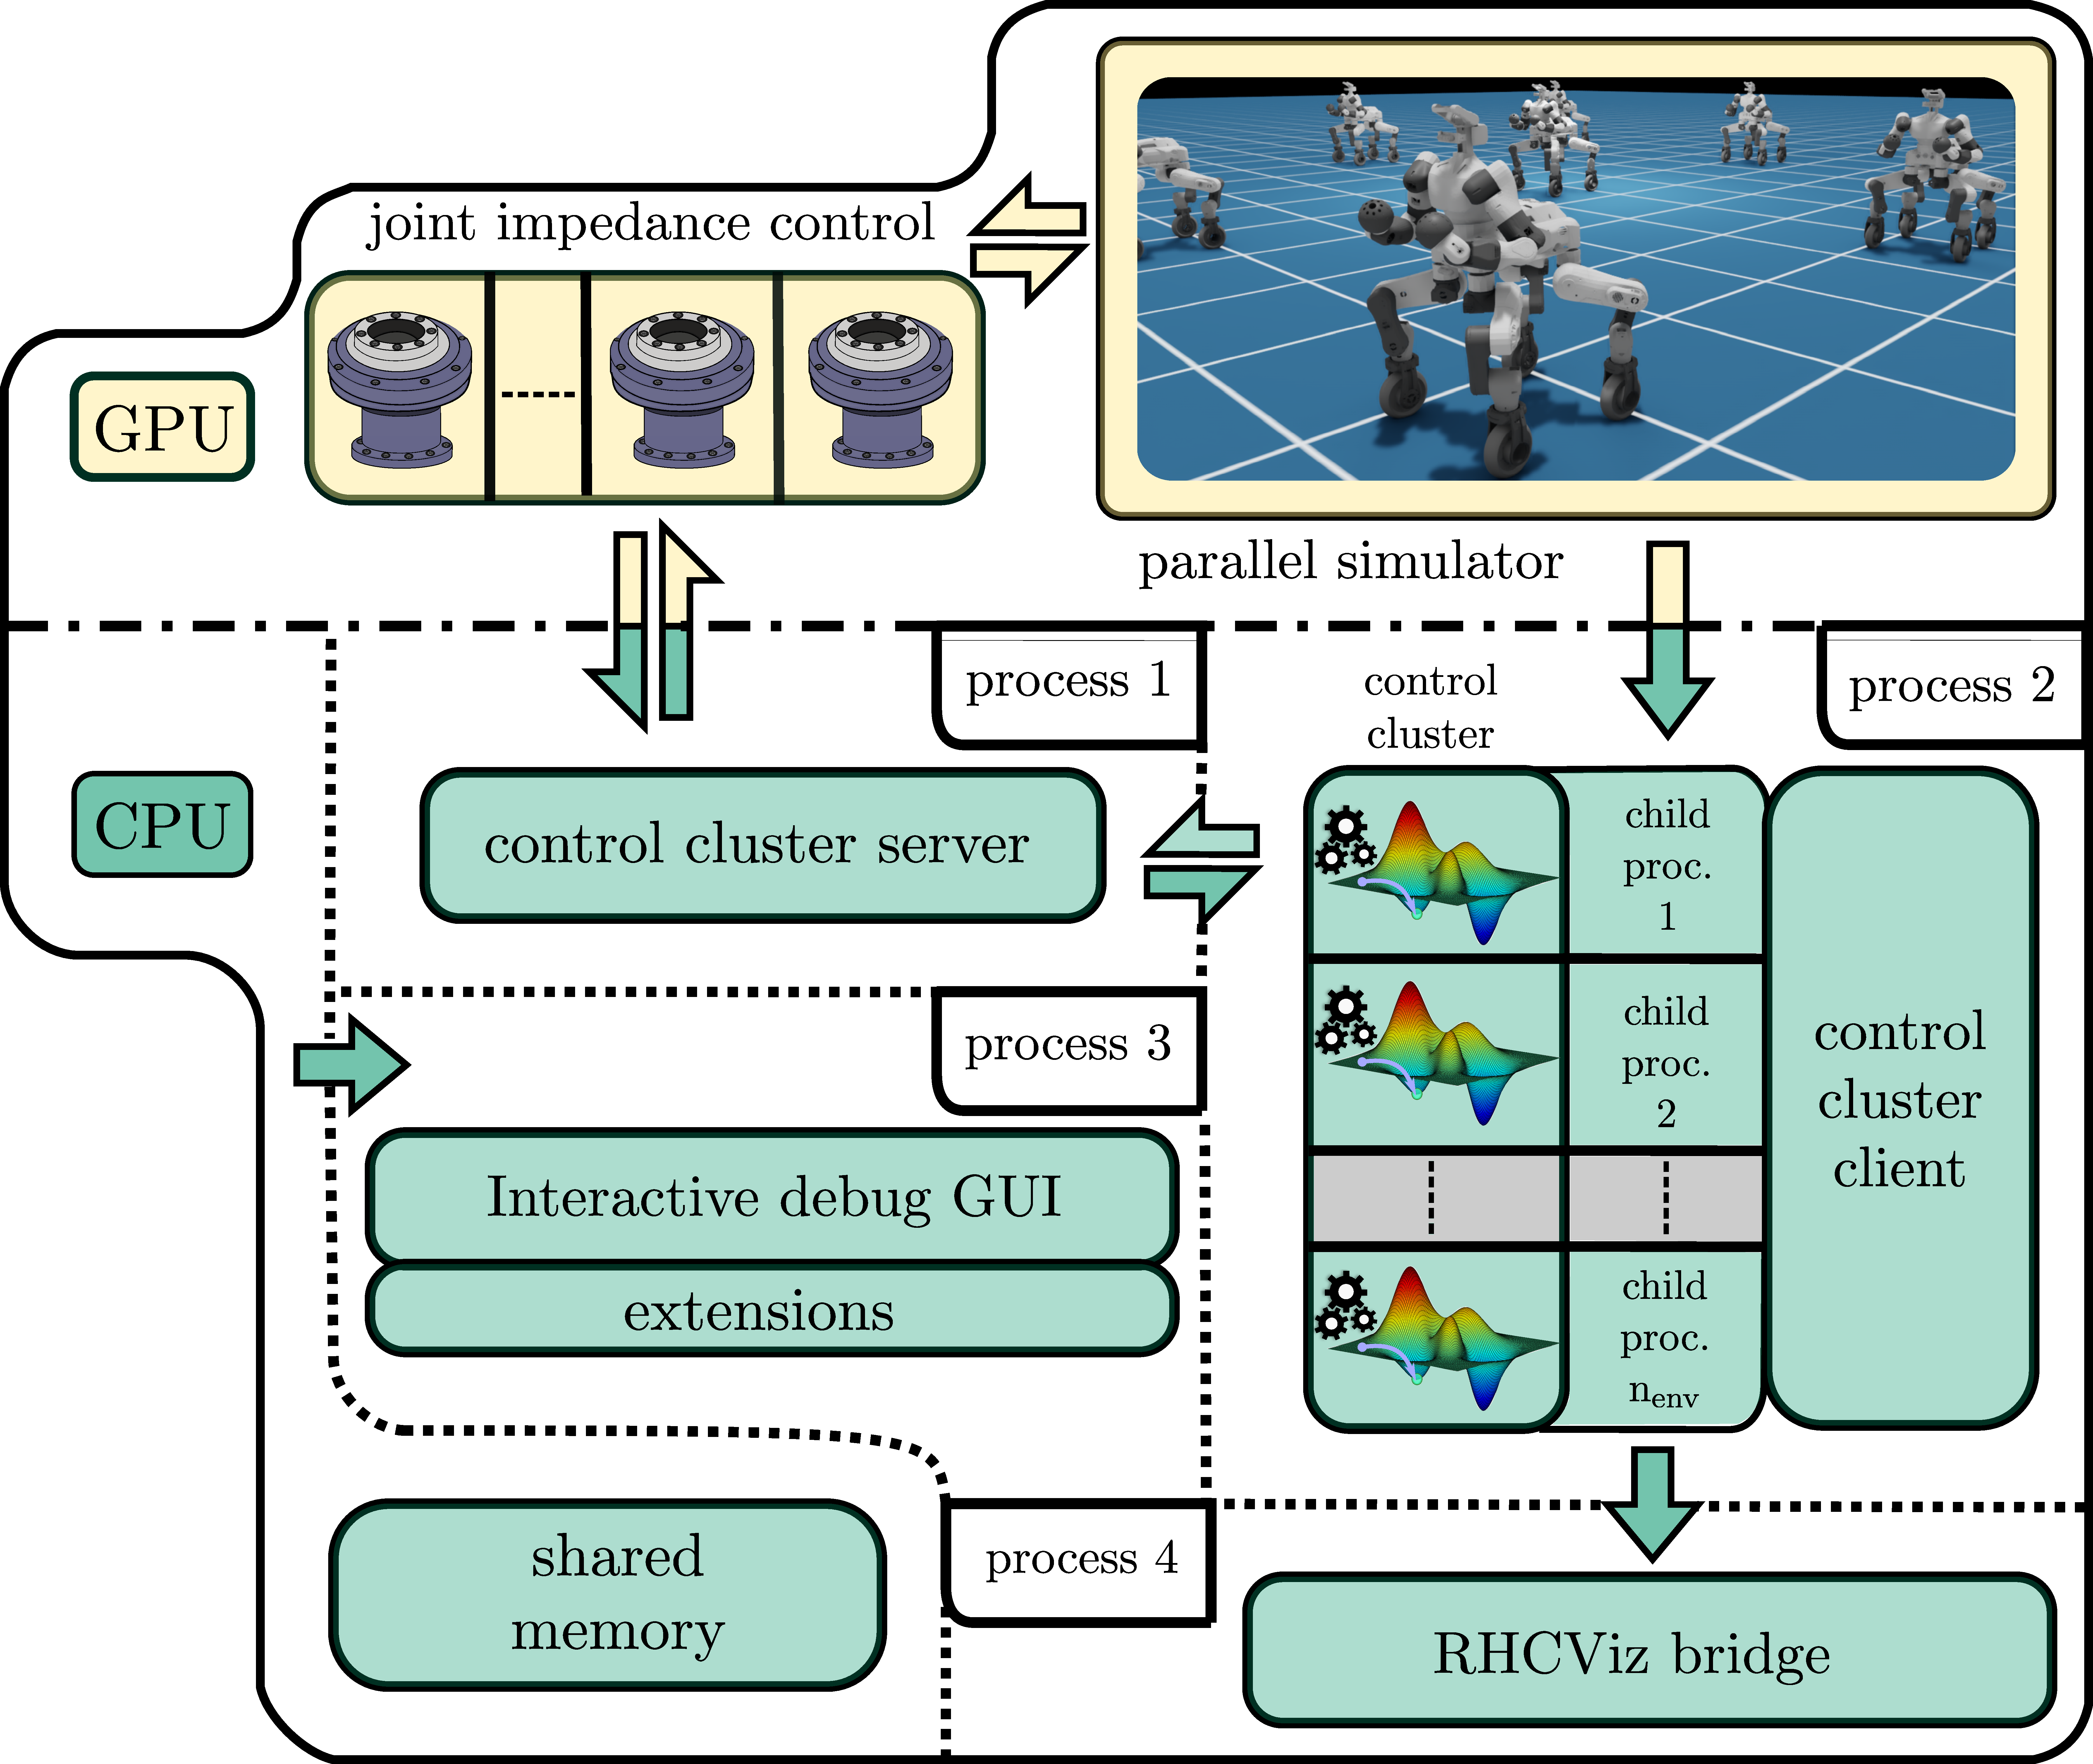
\includegraphics[width=0.8\textwidth]{docs/imgs/cocluster_arch_full.pdf}
	\end{figure}
	Training env implemented separately wrt simulation environment. One train env step = one cluster step = n simulation steps, depending on the cluster rate.
	Simulation runs parallel wrt cluster solution (more efficient and realistic).
	RHC interfaces with robot thorugh a joint impedance controller. A set of debug tools allow to perform easy reward tuning/inspection of the simulator/RHC,etc..
\end{Large}